\documentclass[a4paper]{article}

\usepackage{INTERSPEECH2021}

\title{Rus1K: Russian Dataset for Speech Research}
\name{Nikolay Karpov$^1$, Co-author Name$^2$}
%The maximum number of authors in the author list is twenty. If the number of contributing authors is more than twenty, they should be listed in a footnote or in acknowledgement section, as appropriate.
\address{
  $^1$Sber, Russia\\
  $^2$Co-author Affiliation}
\email{karpnv@gmail.com, coauthor@company.com}

\begin{document}

\maketitle
% 
\begin{abstract}
 
  This paper introduces Russian language dataset called Rus1K, a large scale corpus suitable for speech research. The dataset mainly consists of audio recorded and manually annotated on the crowd-sourcing platform. Total duration of audio is about 1200 hours. We have made the corpus freely available for download, along with prepared acoustic-model. It's quality evaluated with pre-built language model and transfer learning tricks. 
  
  
\end{abstract}
\noindent\textbf{Index Terms}: speech recognition, open dataset, Russian language, speech corpus

\section{Introduction}
 We believe that open data is a one of the key drivers of recent success in the field of artificial intelligence. In particular automatic speech recognition (ASR) algorithms become much better and more robust resent years. New algorithms allows to create conversational systems with good user experience so that such technologies become more popular. It makes a basement for many new business ideas, disruptions of traditional strategies and benefits for innovators.
  
 Despite the existence of outstanding initiatives such as MLS dataset \cite{pratap2020mls} there is a luck of manually annotated large scale speech corpuses in Russian that is freely available and suitable for training and testing speech recognition systems.
 
 This article is dedicated to present our new open large scale speech dataset. Example script to train on this data is available in the open source NeMo toolkit \cite{kuchaiev2019nemo}. It shows quality of acoustic models with language model and without it. We also demonstrate improvement using pre-trained English acoustic models. The highlights of this paper are following:
\begin{enumerate}
\item Open audio corpus with 1200 hours of manually annotated Russian speech.
\item Example Acoustic model trained on our corpus.
\item Example Language model trained on open data set.
\item Transfer Learning empirical results
\end{enumerate}

Section 2 presents the related works that inspired us to share our corpus. In Section 3 we describe the process we used to build the corpus. Section 4 describes the structure of the dataset. Section 5 presents acoustic model trained on this dataset and language model, which we make available with this corpus. Finally in Section 6 we present some experimental results on transfer learning, using pre-trained English acoustic model.

\section{Related Work}

There are few large scale data collections for speech recognition is available now. 

\subsection{Mono-lingual ASR datasets}

Let us mention only few mono-lingual datasets which we think are most important in the field of Russian speech recognition.

First is LibriSpeech  \cite{panayotov2015librispeech} which  includes about 1000 hours of English audio-books. It is derived from the big LibriVox dataset,  distributed under an open license. Second is an audio part of Wall Street Journal (WSJ) corpus \cite{paul1992design} which contains about 400 hrs. of speech data. These two datasets usually used to evaluate state of the art (SoTA) speech recognition algorithms.

Open-STT is the only Russian language large-scale dataset. It consists of more then 15000 hours \cite{veysov2020towardimagenetstt}. Unfortunately its annotation is not manually created. Transcriptions are derived by doing  alignment or ASR system. 

\begin{table}[th]
  \caption{Content of Open STT Russian corpus}
  \label{tab:openstt}
  \centering
  \begin{tabular}{ llcr }
    \toprule
    Domain & Annotation & Utterances & Hours~~~  \\
    \midrule
    Radio &     Alignment & 8.3M & 11 996 ~~~  \\
    Public Speech & Alignment  & 1,7M & 2 709 ~~~ \\
    YouTube & Subtitles  & 2,6M & 2 117 ~~~ \\
    Audiobooks & Alignment  & 1,3M & 1 632 ~~~ \\
    Calls & ASR  & 695K & 819 ~~~ \\
    Other & TTS  & 1.9M & 835 ~~~ \\
    \bottomrule
  \end{tabular}
\end{table}

\subsection{Multi-lingual ASR datasets}

VoxForge languages, but remains low-scale (about 300 hours in total).


CommonVoice [4], a more scalable solution, with more than 30 languages available, which keeps growing with 4500 (validated) hours currently available.


MLS \cite{pratap2020mls} is a large-scale multilingual dataset for speech research like a LibriSpeech derived from LibriVox dataset and consists of 8 languages, including about 44.5K hours of English and a total of about 6K hours for other languages.

multi-lingual speech gathering efforts are being conducted:  (ii) 

\section{Data collection pipeline}

This section describes the main steps during data collection and preparation. It includes two stages:

\subsection{Stage 1}

All figures must be centered on the column (or page, if the figure spans both columns). Figure captions should follow each figure and have the format given in Figure~\ref{fig:speech_production}.

Figures should be preferably line drawings. If they contain gray levels or colors, they should be checked to print well on a high-quality non-color laser printer.

\subsection{Stage 2}
\subsubsection{subsubsection}
Graphics (i.\,e., illustrations, figures) must not use stipple fill patterns because they will not reproduce properly in Adobe PDF. Please use only SOLID FILL COLORS.

Figures which span 2 columns (i.\,e., occupy full page width) must be placed at the top or bottom of the page.

\section{Dataset  overview}

\begin{itemize}
\item 1104330 train files
\item 10000 validation files 
\end{itemize}

An example of a table is shown in Table~\ref{tab:example}. 

\begin{table}[th]
  \caption{Train set}
  \label{tab:example}
  \centering
  \begin{tabular}{ r@{}l  r }
    \toprule
    \multicolumn{2}{c}{\textbf{Domain}} & \multicolumn{1}{c}{\textbf{Number of files}} \\
    \midrule
    & Portal & 124511~~~             \\
    & Crowd & 979819~~~               \\

    \bottomrule
    & Total  & 1104330~~~              \\
  \end{tabular}
  
\end{table}


\begin{table}[th]
  \caption{Test set}
  \label{tab:example}
  \centering
  \begin{tabular}{ r@{}l  r }
    \toprule
    \multicolumn{2}{c}{\textbf{Domain}} & \multicolumn{1}{c}{\textbf{Number of files}} \\
    \midrule
    & Portal & 1916~~~  \\
    & Crowd  & 10000~~~ \\
    \bottomrule
    & Total  & 11916~~~ \\
  \end{tabular}
  
\end{table}

\section{Acoustic and Language model}

The best way to show the quality of data is to train some model on it and estimate quality of the model. We train an acoustic model on the training part of data end evaluate it on the test one with and without language model.

\subsection{Acoustic model}
Training from scratch 

Quartznet \cite{kriman2020quartznet} 

Equations should be placed on separate lines and numbered. Examples of equations are given below. Particularly, 
Table \ref{tabular:Quartznet}
 
\begin{table}[t]
  \caption{QuartzNet Architecture. The model starts with a
conv layer C1 followed by a sequence of 5 groups of blocks.
Blocks in the group are identical, each block Bk consists of R
time-channel separable K-sized convolutional modules with
C output channels. Each block is repeated S times. The model
has 3 additional conv layers (C2, C3, C4) at the end.}
  \label{tabular:Quartznet}
  \centering
  \begin{tabular}{ccccc}
    \toprule
    \textbf{Block}  & \textbf{R} & \textbf{K} & \textbf{C} & \textbf{S 15x5}     \\
    \midrule
    $C_1$  & 1 & 33 & 256 &  1   \\
    \midrule
    $B_1$  & 5 & 33 & 256 &  3  \\
    $B_2$  & 5 & 39 & 256 &  3  \\
    $B_3$  & 5 & 51 & 512 &  3            \\
    $B_4$  & 5 & 63 & 512 &  3            \\
    $B_5$  & 5 & 75 & 512 &  3            \\
    \midrule
    $C_2$  & 1 & 87 & 512 &  1            \\
    $C_3$  & 1 & 1 & 1024 &  1            \\
    $C_4$  & 1 & 1 & $\|labels\|$ &  1     \\
    \bottomrule
    \textbf{Params,M}  &  &  & &  18.9     \\
  \end{tabular}
\end{table}


\subsection{Language model}

We create a language model using Russian part of the Common Crawl dataset and KenLM Language Model Toolkit \cite{heafield-2011-kenlm}. The Common Crawl is a repository of web crawl data that can be accessed and analyzed by anyone. KenLM Toolkit allows to make vary fast ngram language model.


For ease of formatting, please use the styles listed in Table 2. The styles are defined in this template file and are shown in the order in which they would be used when writing a paper. When the heading styles in Table 2 are used, section numbers are no longer required to be typed in because they will be automatically numbered by Word. Similarly, reference items will be automatically numbered by Word when the ``Reference'' style is used.

\begin{table}[t]
  \caption{Language Model Influence}
  \label{tab:word_styles}
  \centering
  \begin{tabular}{lrr}
    \toprule
    \textbf{Model}      & \textbf{crowd}     & \textbf{portal}    \\
    \midrule
    20K without LM   &  4.62\%    & 15.86\%                                \\
    20K  with LM     & 4.86\%       & 12.57\%                         \\

    \bottomrule
  \end{tabular}
\end{table}

If your Word document contains equations, you must not save your Word document from ``.docx'' to ``.doc'' because when doing so, Word will convert all equations to images of unacceptably low resolution.

\section{Transfer Learning}

Transfer learning is a key element for recent success of neural networks, so it is widely used. For instance pre-trained model on the ImageNet in the computer vision or pre-trained Bert in the natural language processing fields. 


Table \ref{tabular:Quartznet} 

\begin{table}[t]
  \caption{Transfer Learning Influence}
  \label{tab:word_styles}
  \centering
  \begin{tabular}{lrr}
    \toprule
    \textbf{Model}      & \textbf{crowd}     & \textbf{portal}    \\
    \midrule
    10K from scratch   &  28.84\%   & 52.82\% \\
    10K from en    & 5.095\%       & 17.13\%  \\
    \midrule
    20K from scratch   &  26.24\%   & 50.82\% \\
    20K from en    & 4.63\%       & 15.82\% \\
    \bottomrule
  \end{tabular}
\end{table}


Transfer Learning Figure \ref{fig:wer10k} and \ref{fig:wer20k}

\begin{figure}
    \centering
    \subfigure{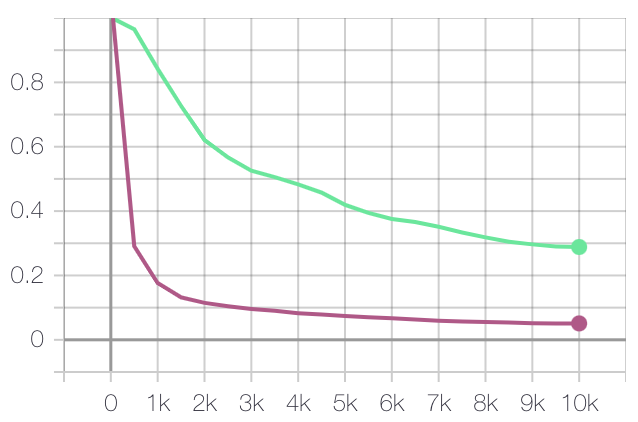
\includegraphics[width=0.49\linewidth]{LaTeX/img/crowd10k.png}} 
    \subfigure{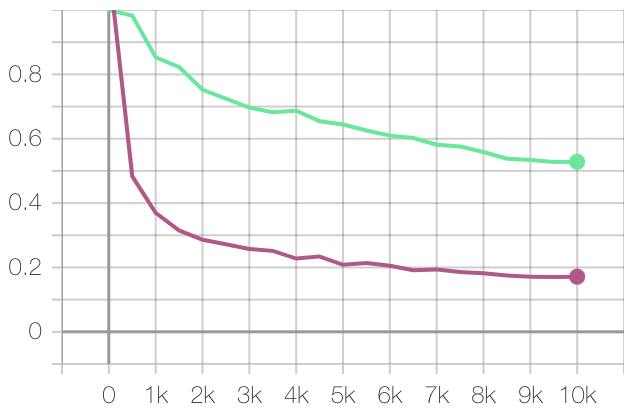
\includegraphics[width=0.49\linewidth]{LaTeX/img/portal10k.png}} 
    \caption{Transfer learning influence with 10K steps (a) Crowd 5.095\% vs 28.84\% (b) Portal 17.13\% vs 52.82\%}
    \label{fig:wer10k}
\end{figure}


\begin{figure}
    \centering
    \subfigure{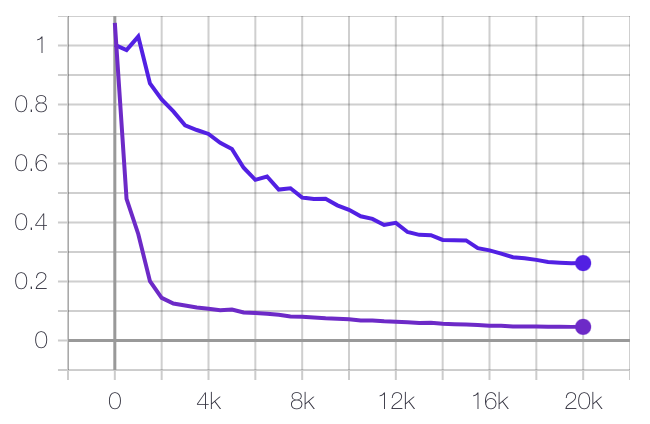
\includegraphics[width=0.49\linewidth]{LaTeX/img/crowd20k.png}} 
    \subfigure{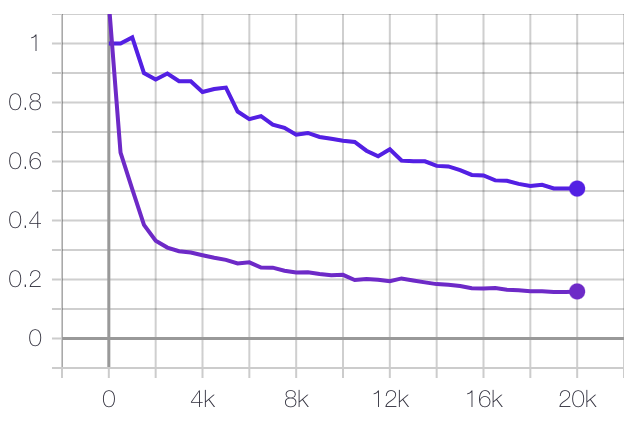
\includegraphics[width=0.49\linewidth]{LaTeX/img/portal20k.png}} 
    \caption{Transfer learning influence with 20K steps (a) Crowd 4.63\% vs 26.24\%  (b) Portal 15.95\% vs 50.82\%}
    \label{fig:wer20k}
\end{figure}





\section{Conclusions}

Authors must proofread their PDF file prior to submission to ensure it is correct. Authors should not rely on proofreading the Word file. Please proofread the PDF file before it is submitted.

\section{Acknowledgements}

The ISCA Board would like to thank the organizing committees of the past INTERSPEECH conferences for their help and for kindly providing the template files. \\
Note to authors: Authors should not use logos in the acknowledgement section; rather authors should acknowledge corporations by naming them only.


\bibliographystyle{IEEEtran}

\bibliography{mybib}

% \begin{thebibliography}{9}
% \bibitem[1]{Davis80-COP}
%   S.\ B.\ Davis and P.\ Mermelstein,
%   ``Comparison of parametric representation for monosyllabic word recognition in continuously spoken sentences,''
%   \textit{IEEE Transactions on Acoustics, Speech and Signal Processing}, vol.~28, no.~4, pp.~357--366, 1980.
% \bibitem[2]{Rabiner89-ATO}
%   L.\ R.\ Rabiner,
%   ``A tutorial on hidden Markov models and selected applications in speech recognition,''
%   \textit{Proceedings of the IEEE}, vol.~77, no.~2, pp.~257-286, 1989.
% \bibitem[3]{Hastie09-TEO}
%   T.\ Hastie, R.\ Tibshirani, and J.\ Friedman,
%   \textit{The Elements of Statistical Learning -- Data Mining, Inference, and Prediction}.
%   New York: Springer, 2009.
% \bibitem[4]{YourName17-XXX}
%   F.\ Lastname1, F.\ Lastname2, and F.\ Lastname3,
%   ``Title of your INTERSPEECH 2021 publication,''
%   in \textit{Interspeech 2021 -- 20\textsuperscript{th} Annual Conference of the International Speech Communication Association, September 15-19, Graz, Austria, Proceedings, Proceedings}, 2020, pp.~100--104.
% \end{thebibliography}

\end{document}
